%% LaTeX2e class for student theses
%% sections/content.tex
%% 
%% Karlsruhe Institute of Technology
%% Institute for Program Structures and Data Organization
%% Chair for Software Design and Quality (SDQ)
%%
%% Dr.-Ing. Erik Burger
%% burger@kit.edu
%%
%% Version 1.3.3, 2018-04-17

\chapter{Background}
\label{ch:Background}

% TODO improve examples. abandon the dream of one grand example for everything – now is better than never

% TODO longer introductory paragraph?
This chapter provides background information
on several concepts that are important to the rest of this thesis.
The sections below are not intended to be comprehensive introductions to the respective topics,
but focus on the aspects that are necessary to understand the thesis.
More information can be found in the bibliography. % TODO this sentence feels weird. the bibliography doesn’t have more information, it just points you to it

\section{Wikidata}
\label{sec:Background:Wikidata}

\gls{Wikidata} \cite{Vrandecic:2014:WFC:2661061.2629489} % TODO is that the best place for this \cite{}?
is a free knowledge base
and part of the \gls{Wikimedia} family of sister projects,
the most famous of which is \gls{Wikipedia}, the free encyclopedia.
Its contents are created, maintained and managed by the \gls{Wikidata} community,
most of whose members are volunteers,
as well as the members of \gls{Wikidata}’s sister projects, e.~g. \gls{Wikipedia}.
Anyone can contribute to \gls{Wikidata},
but the community ensures the quality of the contents with various quality control mechanisms.
Providing another such mechanism is part of the motivation for this thesis.

Information on \gls{Wikidata} is collected in \glspl{item},
which represent things or concepts:
there are \glspl{item} for individual persons,
for cities, states, geographical features,
for organizations and corporations,
\glspl{item} for books, films, newspapers, journals, scientific articles,
for abstract concepts, phenomena, emotions, philosophical movements, political orientations,
\glspl{item} for conceptual hierarchies, parent classes, biological taxa,
and even \glspl{item} for fictional characters, places, or other entities.

All of these \glspl{item} follow the same structure.
They are identified by their \gls{item ID},
a consecutive number prefixed with the letter “Q”
(e.~g. \Q{Q188709} for Beethoven’s Symphony No. 5).
They can have a \gls{label}, \gls{description}, and search \glspl{alias} in various languages:
for example, \Q{Q7251} is labeled “Alan Turing” in English
but «\foreignlanguage{russian}{Алан Тьюринг}» in Russian;
is described as a “British mathematician, logician, cryptanalyst, and computer scientist” in English;
and may also be found under search aliases like “Alan M. Turing”, “Alan Mathison Turing” or simply “Turing”.
They also have a set of \glspl{sitelink}
(links to pages about the same concept in various other \gls{Wikimedia} projects –
\gls{Wikipedia} articles, \gls{Wikiquote} pages, \gls{Wikimedia Commons} galleries, etc.),
and most importantly, a set of \glspl{statement}.

The \glspl{statement} are where most of the information in \gls{Wikidata} is stored.
They consist of a \gls{property}, such as “place of birth” or “author” or “population”,
and a value, which can be a reference to another \gls{item}, a quantity, a point in time, a piece of text,
or a few other possible types.
A \gls{statement} can also have \glspl{qualifier}
(further property-value pairs, e.~g. clarifying when or where the statement is valid)
and \glspl{reference} (sets of property-value pairs, listing sources for the \gls{statement}),
but those are mostly ignored in the context of this thesis.
\Glspl{property} are also identified by an ID, their \gls{property ID}
(prefixed with the letter “P” instead of “Q”),
and can also have \glspl{label}, \glspl{description} and \glspl{alias} in different languages:
for example, \P{P31} is labeled “instance of” in English
and „\foreignlanguage{ngerman}{ist ein(e)}“ in German.
The \glspl{label} and \glspl{description} are necessary to understand the meaning of \glspl{statement},
but they are not themselves part of the \glspl{statement}:
\glspl{statement} only list references to \gls{property} and \glspl{item ID},
making most of the information in \gls{Wikidata} language-agnostic \cite{Kaffee:2017:GBA:3125433.3125465}.

% TODO split the following paragraph into multiple, under a dedicated subsection?
\Cref{fig:montblanc} shows two screenshots of the same \gls{Wikidata} \gls{item},
\QL{Q761735}{Montblanc}, viewed in different languages.
% TODO mention the revision ID? 704641959
The page structure is the same regardless of language:
first, there is a heading, showing the \gls{label} in the current language and the \gls{item ID};
below it on the left side is the “term box”,
listing \glspl{label}, \glspl{description} and \glspl{alias} in several languages relevant to the user;
below that is the list of \glspl{statement};
to the right are lists of \glspl{sitelink} for different \gls{Wikimedia} projects.
The screenshots are truncated
(the page has also been lightly edited for the screenshots
to remove some spacing and a few less relevant page elements)
and do not show the full list of \glspl{statement},
but the \glspl{statement} pictured are:
\begin{itemize}
\item A \gls{statement} for the \gls{property} \P{P31},
  where the value is an \gls{item}, \Q{Q33146843}.
\item A \gls{statement} for the \gls{property} \P{P18},
  where the value is a media file on \gls{Wikimedia Commons}.
  Image credit:
  \href{https://commons.wikimedia.org/wiki/User:Mariarosafg}{Mariarosafg}
  (\url{https://commons.wikimedia.org/wiki/File:Ciutat_de_Montblanc.jpg}),
  “Ciutat de Montblanc”,
  \url{https://creativecommons.org/licenses/by-sa/3.0/legalcode}
\item Two \glspl{statement} for the \gls{property} \P{P1448},
  where the values are monolingual text strings.
  Both \glspl{statement} also have \glspl{qualifier} and \glspl{reference}.
\end{itemize}
In \cref{fig:montblanc-en},
the \gls{item} is viewed as an anonymous user in the default English language
(German is shown as a second language in the term box
because the request was made from a German IP address;
logged in users can configure which languages they want to be shown here).
In \cref{fig:montblanc-ca},
the \gls{item} is viewed as an anonymous user, explicitly requested in the Catalan language:
notice that all \gls{property} and \gls{item} \glspl{label} are now different.

\begin{figure}
  \caption{Two screenshots of the same \gls{item} viewed in different languages.}
  \label{fig:montblanc}
  \begin{subfigure}{\textwidth}
    \caption{The \gls{item} viewed as an anonymous user in the default English language.}
    \label{fig:montblanc-en}
    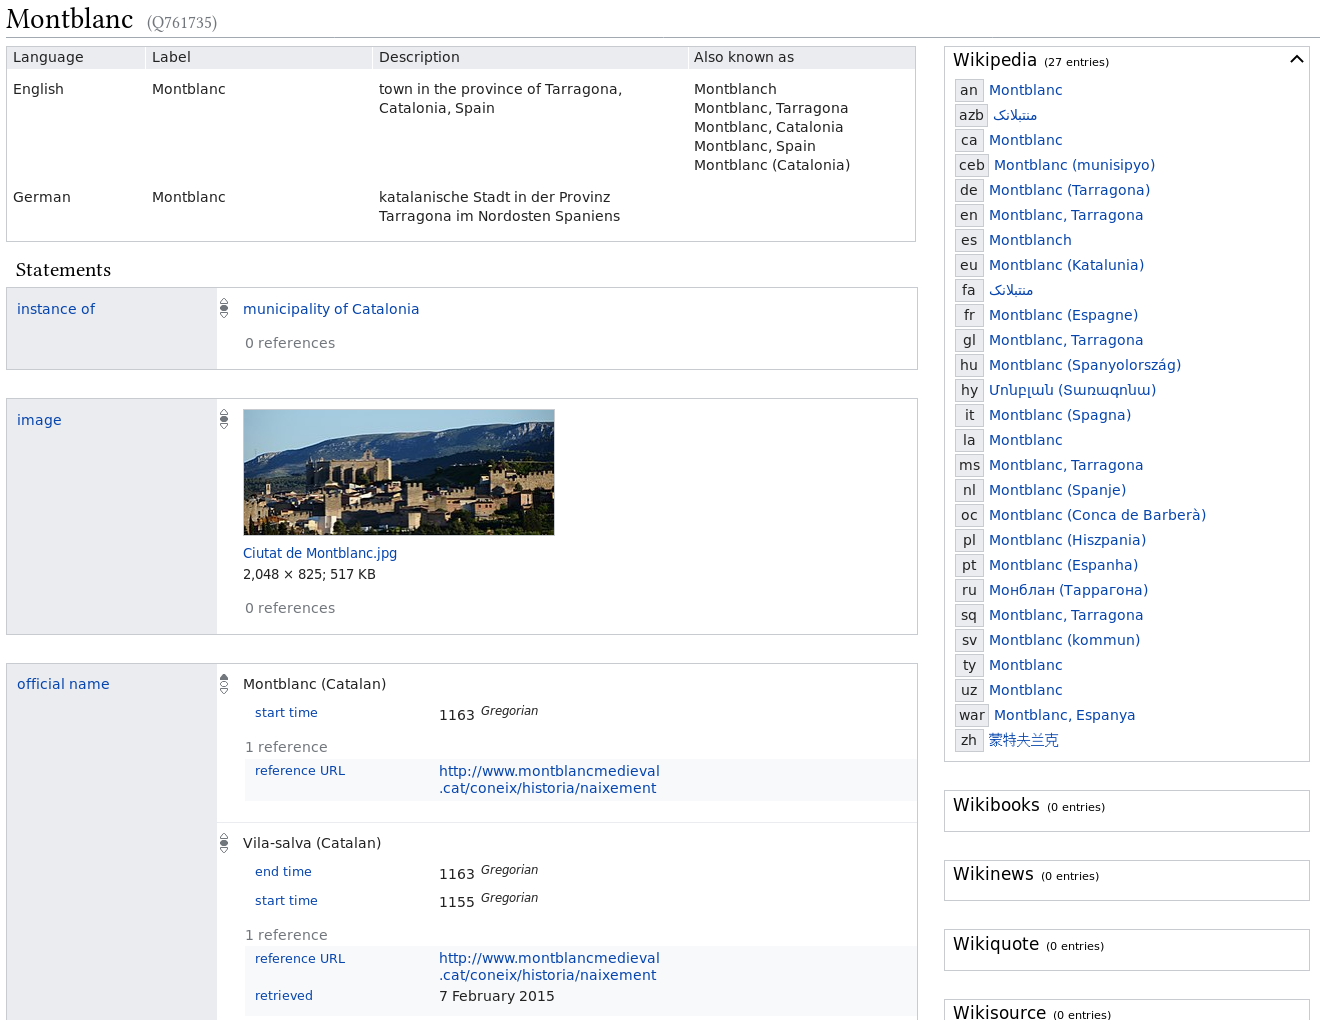
\includegraphics[width=\textwidth]{screenshots/montblanc-en}
  \end{subfigure}
\end{figure}
\begin{figure}\ContinuedFloat
  \begin{subfigure}{\textwidth}
    \caption{The \gls{item} viewed as an anonymous user, explicitly requested in the Catalan language.}
    \label{fig:montblanc-ca}
    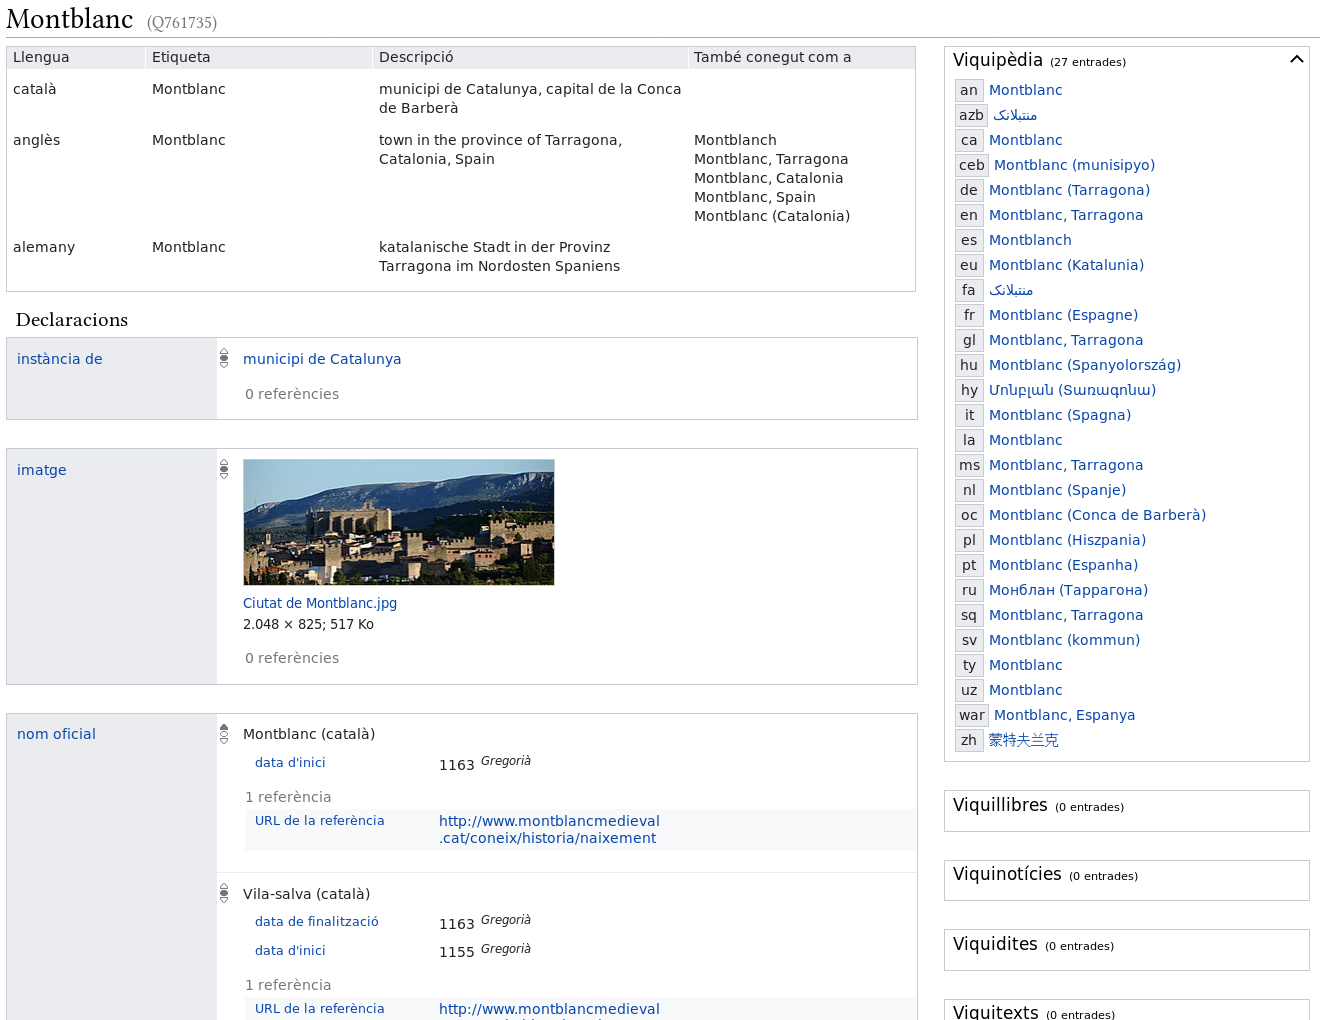
\includegraphics[width=\textwidth]{screenshots/montblanc-ca}
  \end{subfigure}
\end{figure}

It is vital to observe that there is no kind of \gls{schema} inherent to the \gls{Wikidata} data model.
Any \gls{property} can be used on any \gls{item}:
nothing in the software stops one from adding, say,
a “date of birth” \gls{statement} to an \gls{item} for a lake,
or a “parent taxon” \gls{statement} to an \gls{item} for a movie teaser poster.
The community has several ways to describe \glspl{schema} to varying degrees of formality
(such as \gls{property} lists on WikiProject pages or the property constraints system),
but they are all realized by community consensus,
not enforced by the \gls{Wikidata} software.
The great flexibility which this lends to the community
is considered to be one of \gls{Wikidata}’s greatest strengths \cite{vrandecic-restricting-the-world},
and though the use of \gls{shex}
on \gls{Wikidata} will provide another,
highly formal way to describe \glspl{schema},
it is not intended to change this fundamental operating principle of \gls{Wikidata}. % TODO awkward passive voice

\gls{Wikidata}’s data model, as described above,
is not directly related to \gls{rdf}.
However, to enable usage of \gls{rdf} technologies and interoperation with \gls{rdf}-based data sets,
\gls{Wikidata}’s data is exported to \gls{rdf}:
% TODO link to Help:Data access and query.wikidata.org? if yes, \href or \url?
the data about any \gls{item} can be downloaded in various \gls{rdf} formats through a linked data interface, % TODO *the* linked data interface?
and a full, up-to-date \gls{rdf} export of \gls{Wikidata} is available in \gls{wdqs},
a \acrshort{sparql} endpoint to which anyone may submit queries.
However, this interface is export-only:
it is not possible to edit \gls{Wikidata} via \gls{rdf}.

% TODO explain some fundamental properties? P31, P279?

\section{RDF}
\label{sec:Background:RDF}

\acrfull{rdf}
\cite{Lanthaler:14:RCA}
is a framework for describing and working with linked data.
In \gls{rdf}, information is arranged in \gls{subject}-\gls{predicate}-\gls{object} \glspl{triple},
such as “<Alan Turing> <is a> <human>”
or “<Lima> <was founded in> <18 January 1535>”.
All three elements of a \gls{triple} are typically \glspl{resource},
identified by an \gls{iri} like \url{http://example.com/Alan_Turing} or \url{http://www.wikidata.org/entity/Q5},
but the \gls{object} of a \gls{triple} can also be some other kind of value,
such as a textual, numerical or other literal
(e.~g. the date literal “18 January 1535” above). % TODO blank nodes are elided for brevity, but perhaps rephrase this to make sure the text isn’t factually wrong
A collection of such \glspl{triple} forms a directed, labeled graph,
where the \glspl{triple} describe individual edges
and the nodes are the \glspl{subject} and \glspl{object} of the \glspl{triple}:
\glspl{triple} with the same \gls{subject} constitute different outgoing arcs from the same node.
This graph can then be queried using the \acrlong{sparql} \cite{9569543}. % TODO is SPARQL really important enough to be mentioned here, and nothing else?
For a more detailed introduction,
see the RDF 1.1 Primer \cite{Schreiber:14:RP}.
% TODO the previous sentence should probably be at the end of the section, not of the paragraph

To improve readability, the \glspl{iri} identifying a \gls{resource} are usually abbreviated using \emph{prefixes}:
for example, once the prefix \prefix{wd:} has been defined to mean \url{http://www.wikidata.org/entity/},
the \glspl{iri} \url{http://www.wikidata.org/entity/Q7251} and \url{http://www.wikidata.org/entity/Q5}
can be abbreviated as \PName{wd:Q7251} and \PName{wd:Q5}.
The rest of this thesis will use the following prefixes,
also given in \cref{listing:prefixes}:

\begin{description}
\item[\PName{wd:}] A \gls{Wikidata} \gls{item}, like \PName{wd:Q7251}.
\item[\PName{wdt:}] Predicate for a triple representing a \gls{Wikidata} \gls{statement}, e.~g. \PName{wdt:P31}.
\item[\PName{rdf:}] Part of the RDF Schema vocabulary (see below).
\item[\PName{rdfs:}] Part of the RDF Schema vocabulary.
  (The distinction between \PName{rdf:} and \PName{rdfs:} is “a somewhat annoying historical artifact” \cite{Schreiber:14:RP}
  with no real significance today.)
\item[\PName{ex:}] An example entity.
  Following the naming conventions of schema.org \cite{schema.org-old-extension},
  types and entities are in upper camel case (\PName{ex:Human})
  while predicates are in lower camel case (\PName{ex:dateOfBirth}).
\end{description}

\begin{lstfloat}
\begin{lstlisting}[language=sparql]
PREFIX wd: <http://www.wikidata.org/entity/>
PREFIX wdt: <http://www.wikidata.org/prop/direct/>
PREFIX rdf: <http://www.w3.org/1999/02/22-rdf-syntax-ns#>
PREFIX rdfs: <http://www.w3.org/2000/01/rdf-schema#>
PREFIX ex: <http://shex.example/>
\end{lstlisting}
\caption{Default prefixes used in this thesis.}
\label{listing:prefixes}
\end{lstfloat}

While \gls{rdf} can be used with any \gls{resource} \glspl{iri},
one of its strengths is the ability to reuse the same \emph{vocabularies}
(effectively, sets of \glspl{resource})
in many different graphs.
For example, many graphs use the same \gls{predicate}, \PName{rdfs:label},
to link a \gls{resource} to a human-readable version of its name (its label);
a tool based on \gls{rdf} can thus offer human-readable names for \glspl{resource} from all these graphs
without requiring any specific knowledge about them,
and the graphs are more useful when used in combination.
One common vocabulary is RDF Schema \cite{Guha:14:RS}, % acronym for RDFS?
which among others provides two important predicates:
\PName{rdf:type} and \PName{rdfs:subClassOf}.
\PName{rdf:type} connects an object to its class,
and \PName{rdfs:subClassOf} connects a class to its parent class.
% TODO continue writing: example for rdf:type and rdfs:subClassOf

\section{Shape Expressions}
\label{sec:Background:ShEx}

% TODO somewhere, there needs to be a clear explanation why it’s so okay for us to constantly discard type links. here? not sure
% TODO example for validation

\acrfull{shex} \cite{shex}
is a standard for describing data shapes within an \gls{rdf} graph,
developed by the \gls{shex} Community Group under the umbrella of the \gls{w3c}.
A \gls{shex} \gls{schema} consists of a number of \glspl{shape},
each of which describes the layout of an \gls{rdf} \gls{resource},
called the \gls{focus node}.
The most common notation for \gls{shex} \glspl{schema} is \gls{shexc}, % TODO most common? most convenient? most something else?
and while a full introduction to \gls{shex} and \gls{shexc} is beyond the scope of this thesis,
the relevant elements are described below.

In \gls{shexc}, a \gls{shape} definition begins with the \gls{shape}’s name (an \gls{iri})
and is followed by a block of \glspl{triple constraint} enclosed in curly braces (\lstinline!{}!).
The \glspl{triple constraint} are separated by semicolons (\lstinline{;})
and place restrictions on \glspl{triple} with the \gls{focus node} as the \gls{subject} and a certain \gls{predicate}:
a \gls{triple constraint} consists of the \gls{iri} for the \gls{predicate} and then a constraint on the \gls{object} (the value).
The value constraint can require the value to be a literal with a certain datatype,
expressed directly via the datatype’s \gls{iri},
or it can require the value to be a \gls{resource} matching another \gls{shape},
indicated by that \gls{shape}’s name (an \gls{iri}) following an \lstinline{@} symbol.
The value constraint may be followed by a cardinality for the \gls{triple constraint}:
instead of the default cardinality “must occur exactly once”,
the symbol \lstinline{?} may be appended to signify “zero or one times”
(an optional \gls{triple constraint}),
\lstinline{*} means “zero or more”
(any number of \glspl{triple} with this \gls{predicate} may occur,
but if they do occur, their \glspl{object} must still match the \gls{value constraint}),
and \lstinline{+} means “one or more”.
Multiple possible \glspl{triple constraint} for the same \gls{predicate} can be expressed
by grouping them inside parentheses (\lstinline{()}), separated by vertical bars (\lstinline{|}).

\begin{lstfloat}
\begin{lstlisting}[language=sparql]
ex:CreativeWork {
  ex:title rdf:langString;
  (
    ex:author @ex:Person+ |
    ex:author @ex:Organization
  );
  ex:cites @ex:CreativeWork*;
  ex:publicationDate xsd:dateTime?
}

ex:Person {
  ex:name rdf:langString;
  ex:dateOfBirth xsd:dateTime?
}

ex:Organization {
  ex:name rdf:langString+
}
\end{lstlisting}
\caption{An example \gls{schema} for creative works and their authors.}
\label{listing:shex-example}
\end{lstfloat}

For example, the schema in \cref{listing:shex-example} defines three \glspl{shape}
for creative works and their authors.
It describes a creative work as having a title, a string in a certain language;
being written by one or more persons or an organization;
citing any number of other creative works;
and optionally having been published on a certain date and time.
(Scholarly articles would typically have human authors,
cite multiple works and have a publication date,
whereas a documentation page could be attributed to an organization as a whole
and have no significant citations or publication date.)
A person in this \gls{schema} has exactly one name in one language
(not generally true \cite{falsehoods-programmers-believe-about-names},
but judged by the schema author to be common enough
that violations are more likely to be data entry errors than real exceptions to this rule,
and are therefore worth investigating)
and may have a date of birth, if known.
An organization does not have any properties other than at least one name
(it may have several, e.~g. in different languages or jurisdictions).

% TODO also add example of validation with results?

By default, \gls{shex} \glspl{shape} are not \emph{closed}:
the graph may contain additional \glspl{triple} with the \gls{focus node} as the \gls{subject}
whose \glspl{predicate} do not match any of the \glspl{triple constraint} in the \gls{shape}.
For example, an organization with an \PName{ex:dateOfIncorporation} would still match the \PName{ex:Organization} shape in \cref{listing:shex-example}
even though that \gls{schema} does not mention an \PName{ex:dateOfIncorporation} \gls{predicate} anywhere.
This means that removing all \glspl{triple constraint} with a certain \gls{predicate} from a \gls{shape}
will never cause a previously matching \gls{focus node} to no longer match the \gls{shape}.
% TODO I feel like this is missing one or two sentences at the end

\section{\gls{RDF2Graph}}
\label{sec:Background:RDF2Graph}

% TODO review the layout of the figures here

\gls{RDF2Graph} \cite{vanDam2015}
is a tool to automatically determine the structure of an \gls{rdf} graph
and export it as a \gls{shex} \gls{schema}
(other output formats are also supported).
It relies heavily on the type information of each node and the class hierarchy in the graph,
determining the valid \glspl{predicate} and their value types and cardinalities for each type in the graph.
There is also an optional step to simplify the resulting \gls{schema}.

To discover the structure of an \gls{rdf} graph,
\gls{RDF2Graph} runs a set of queries against a \gls{sparql} endpoint serving that graph.
(This can be a local server, perhaps simply based on a single file containing the graph,
or a remote server.)
It enumerates all the classes that occur in the graph
and then collects all the \glspl{predicate} that are used on instances of each class.
For each \gls{predicate} of each class,
it then gets the types referenced in the values for those \glspl{predicate}
(usually the classes of the referenced nodes,
but values can also be literals or external references),
as well as forward and reverse multiplicity for each such type link.
All this information is stored in a separate \gls{rdf} graph private to \gls{RDF2Graph}.

If the simplification step is enabled,
\gls{RDF2Graph} will afterwards apply some transformations to the structure
based on the hierarchy of the classes involved,
which happens in several steps.
The following description uses the same step numbers as \cite{vanDam2015},
but elides several steps which are mostly implementation details,
which is why the step numbers are not contiguous.
See \cite{vanDam2015} and the \gls{RDF2Graph} source code for the full description.
(In the source code, the steps are counted as sub-steps of the general step 7.4 “simplification”:
for example, step 2 is implemented under a code comment for “7.4.2”.)

% TODO justify somewhere (not sure if in Background) why we are using simplification

In step 2, all \glspl{predicate} from child classes are copied to parent classes,
as outlined in \cref{fig:simplify-7.4.2}.

\begin{figure}[ht]
  \begin{subfigure}[t]{0.45\textwidth}
    \begin{lstlisting}[showlines=true]
A1 extends X {
  a A;
}
A2 extends X {
  a A;
}
B extends X {
  b B;
}
X {}



    \end{lstlisting}
    \caption{Before step 2.}
    \label{fig:simplify-7.4.2-before}
  \end{subfigure}
  \begin{subfigure}[t]{0.45\textwidth}
    \begin{lstlisting}
A1 extends X {
  a A;
}
A2 extends X {
  a A;
}
B extends X {
  b B;
}
X {
  a A;
  b B;
}
    \end{lstlisting}
    \caption{After step 2.}
    \label{fig:simplify-7.4.2-after}
  \end{subfigure}
  \caption[Simplification step 2.]{Simplification step 2 (in pseudo-syntax).}
  \label{fig:simplify-7.4.2}
\end{figure}

Step 3  removes \glspl{predicate} which are only found in a single subclass
from the parent class again.
In the example from \cref{fig:simplify-7.4.2},
the \gls{predicate} \lstinline{a} will be kept in \lstinline{X}
because it occurs in both \lstinline{A1} and \lstinline{A2},
but the \gls{predicate} \lstinline{b} will be dropped
because it only occurs in the single subclass \lstinline{B} –
see \cref{fig:simplify-7.4.3}.

\begin{figure}[ht]
  \begin{subfigure}[t]{0.45\textwidth}
    \begin{lstlisting}
A1 extends X {
  a A;
}
A2 extends X {
  a A;
}
B extends X {
  b B;
}
X {
  a A;
  b B;
}
    \end{lstlisting}
    \caption{Before step 3.}
    \label{fig:simplify-7.4.3-before}
  \end{subfigure}
  \begin{subfigure}[t]{0.45\textwidth}
    \begin{lstlisting}[showlines=true]
A1 extends X {
  a A;
}
A2 extends X {
  a A;
}
B extends X {
  b B;
}
X {
  a A;
}

    \end{lstlisting}
    \caption{After step 3.}
    \label{fig:simplify-7.4.3-after}
  \end{subfigure}
  \caption[Simplification step 3.]{Simplification step 3 (in pseudo-syntax).}
  \label{fig:simplify-7.4.3}
\end{figure}

After that, in step 4 all references which are still found in a parent class
are removed from the child classes, where they are now redundant.
See \cref{fig:simplify-7.4.4} for applying this to the same example.
Note that this step was later disabled, see \cref{sec:RDF2Graph+Wikidata:updates}.

\begin{figure}[ht]
  \begin{subfigure}[t]{0.45\textwidth}
    \begin{lstlisting}
A1 extends X {
  a A;
}
A2 extends X {
  a A;
}
B extends X {
  b B;
}
X {
  a A;
  b B;
}
    \end{lstlisting}
    \caption{Before step 4.}
    \label{fig:simplify-7.4.4-before}
  \end{subfigure}
  \begin{subfigure}[t]{0.45\textwidth}
    \begin{lstlisting}[showlines=true]
A1 extends X {}
A2 extends X {}
B extends X {
  b B;
}
X {
  a A;
}





    \end{lstlisting}
    \caption{After step 4.}
    \label{fig:simplify-7.4.4-after}
  \end{subfigure}
  \caption[Simplification step 4.]{Simplification step 4 (in pseudo-syntax).}
  \label{fig:simplify-7.4.4}
\end{figure}

Step 2 also merges references to parent classes,
as outlined in \cref{fig:simplify-7.4.2-classes}.
The other steps take this into account by respecting subclass relations as well.

\begin{figure}[ht]
  \begin{subfigure}[t]{0.3\textwidth}
    \begin{lstlisting}[showlines=true]
A1 extends A {}
A2 extends A {}
A extends B {}









    \end{lstlisting}
    \caption{The class hierarchy for this example.}
    \label{fig:simplify-7.4.2-classes-hierarchy}
  \end{subfigure}
  \begin{subfigure}[t]{0.3\textwidth}
    \begin{lstlisting}[showlines=true]
M extends X {
  r A1
}
N extends X {
  r A2
}
O extends X {
  r B
}
X {}


    \end{lstlisting}
    \caption{Before step 2.}
    \label{fig:simplify-7.4.2-classes-before}
  \end{subfigure}
  \begin{subfigure}[t]{0.3\textwidth}
    \begin{lstlisting}
M extends X {
  r A1
}
N extends X {
  r A2
}
O extends X {
  r B
}
X {
  r B;
}
    \end{lstlisting}
    \caption{After step 2.}
    \label{fig:simplify-7.4.2-classes-after}
  \end{subfigure}
  \caption[Simplification step 2, with class relations.]{
    Simplification step 2 (in pseudo-syntax), with class relations.
    (This example is independent from the previous example.)
  }
  \label{fig:simplify-7.4.2-classes}
\end{figure}

% TODO I haven’t looked too closely into any of these steps except the very last one,
% which I practically rewrote from scratch.
% Does that show in the text? Do I need to investigate the rest of the ShEx exporter further?
At this point, the information which \gls{RDF2Graph} extracted is available in a private \gls{rdf} graph.
From there, it can be exported into various formats by different exporters.
The \gls{shex} exporter loads parts of these results into a temporary \gls{rdf} database of its own,
applies some transformations to them via \gls{sparql},
converts them to JSON-LD,
further transforms the JSON,
and finally exports the result into \gls{shexc} text via the Jade template engine.

\section{Wikimedia Toolforge}
\label{sec:Background:Toolforge}

% TODO I’m not yet sure if this section is necessary

Wikimedia Toolforge is a hosting environment provided by the Wikimedia Foundation
where trusted members of the \gls{Wikimedia} community may host and develop their “tools” or other work.
Most tools are web-based and reachable under the \href{https://tools.wmflabs.org/}{tools.wmflabs.org} domain,
but it is also possible to run bots or analysis jobs on Toolforge.
Tools can be written in a variety of languages
(e.~g. PHP, Python, Java, JavaScript)
and have access to live replicas of the \gls{Wikimedia} production databases,
data dumps of \gls{Wikimedia} projects,
custom tool-specific databases,
and a Sun Grid Engine job execution system for long-running or resource-intensive tasks.

% TODO more text?
% TODO also mention Cloud VPS? in which case I guess the section heading would be Wikimedia Cloud Services
